\subsection{RQt}
\label{subsec:rqt}

RQt merupakan \emph{framework} \emph{GUI} berbasis Qt \citep{url:qtframework} yang digunakan untuk mengimplementasikan \emph{tools} dalam mengatur \emph{node} yang ada pada ROS 2 \citep{url:rqtoverview}.
RQt memiliki fungsi yang relatif sama dengan \emph{ROS 2 CLI},
  yakni untuk keperluan \emph{debugging} pada sistem komunikasi yang ada pada ROS 2,
  namun RQt ini bekerja secara visual dalam bentuk GUI.

Pada RQt, terdapat beberapa \emph{tools} standar yang dapat digunakan untuk melakukan berbagai macam hal seperti melihat data gambar secara visual,
  melihat hubungan komunikasi antar-\emph{node} dalam bentuk diagram,
  dan lain sebagainya.
Seperti yang terlihat pada Gambar \ref{fig:contohrqtgraph},
  RQt memiliki tools bernama \lstinline{rqt_graph} (\emph{ROS Graph}) yang dapat digunakan untuk melihat hubungan yang ada pada setiap \emph{node} dalam bentuk \emph{topic}, \emph{service}, maupun \emph{action}.

\begin{figure}[ht]
  \centering
  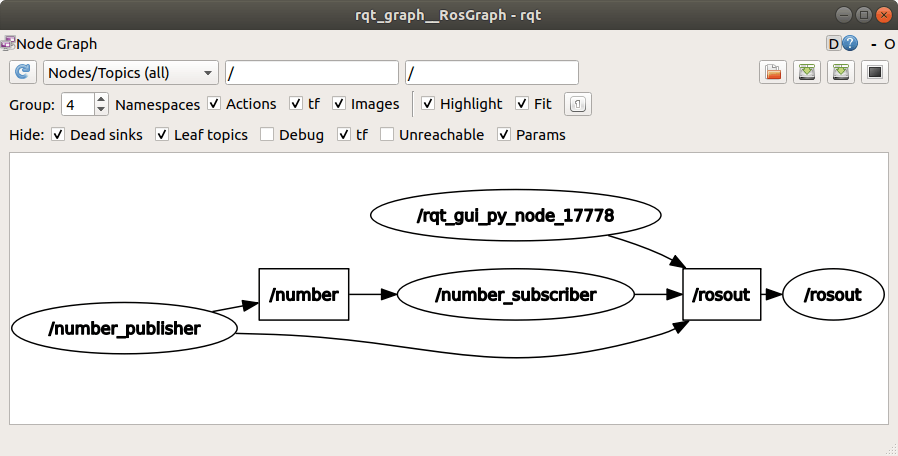
\includegraphics[width=0.95\textwidth,keepaspectratio]{gambar/contoh-rqt-graph.png}
  \caption{Contoh tampilan \lstinline{rqt_graph} (\emph{ROS Graph}) \citep{url:rqtgraphexample}.}
  \label{fig:contohrqtgraph}
\end{figure}

Selain \emph{tools} standar yang sudah disediakan,
  \emph{tools} berbasis GUI pada RQt juga bisa dibuat sendiri maupun diubah menyesuaikan dengan kebutuhan yang diinginkan.
Perubahan tersebut dapat dilakukan melalui \emph{plugin} yang dibuat khusus untuk RQt.
Nantinya \emph{plugin} tersebut dapat disematkan pada \emph{tools} RQt yang dikembangkan dan secara langsung dapat digunakan untuk mengakses sistem komunikasi yang ada pada ROS 2.
